\chapter{Hauptteil}

Sei $G$ ein planer intern 3-zusammenhängender Graph mit Aufhängungen $\{a_1,a_2,a_3\}$. Nehmen wir für einen Moment an, dass wir schon ein SLTR für $G$ gefunden haben, dann hat jeder Knoten $v$ in maximal einen inzidenten Gebiet $f$ einen flachen Winkel, mit $(f,v)$ bezeichnet, und liegt auf einer Geraden. Jedes Gebiet $f$ hat genau drei Ecken, also $deg(f)-3$ flache Winkel. Dies liefert im Umkehrschluss eine notwendige Bedingung für die Existent einer SLTR, indem wir die Knoten den Gebieten zuordnen.

\begin{definition}[FAA]
Sei $G=(V,E,F)$ ein planer Graph, dann ist eine Flache Winkel Zuordnung, im weiteren (nach dem englischen \textit{flat-angle-assignment}) mit FAA bezeichnet, ein Matching zwischen Knoten und Gebieten, sodass:
\begin{itemize}
\item [E1] Jedem Gebiet $f$ sind genau $|f|-3$ Knoten zugeordnet.
\item [E2] Jeder Knoten $v$ ist höchstens einem Gebiet zugeordnet.
\end{itemize}
Für den Fall, dass Aufhängungen gegeben sind, dann fordern wir zusätzlich:
\begin{itemize}
\item [E3] Die inzidenten Knoten des äusseren Gebietes, die keine Aufhängungen sind, müssen dem äusseren Gebiet zugeordnet werden.
\end{itemize}
\end{definition}

\begin{figure}[h]
	\centering
  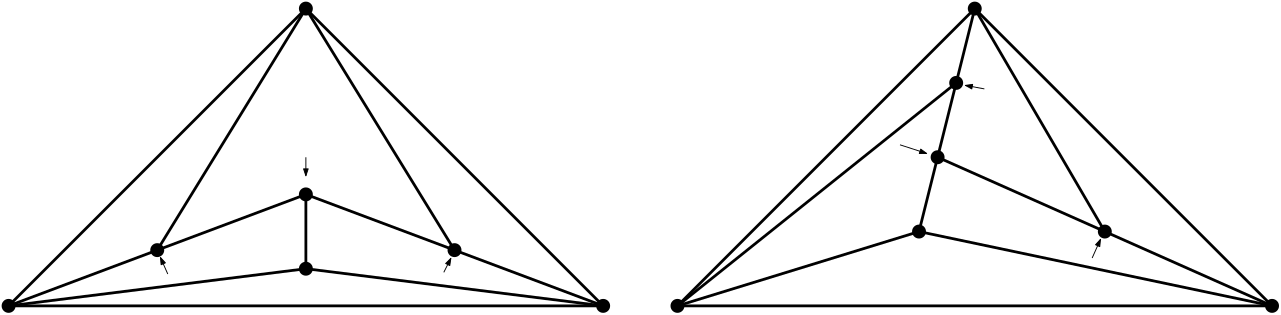
\includegraphics[width=0.9\textwidth]{faa_def.png}
  \caption{Ein planer Graph mit einer SLTR und einem FAA, dass keine SLTR induziert.}
\end{figure}

Ein planer Graph kann also nur dann eine SLTR besitzen, falls mindestens ein FAA existiert, jedoch liefert nicht jedes FAA sofort ein SLTR. Ein FAA, dass zu einer SLTR korrespondiert, wenn also die zugeordneten Winkel des FAA genau die flachen Winkel der SLTR sind, nennen wir von nun an \textit{Gutes-FAA} oder kurz \textit{GFAA}. Unser Ziel wird es sein solche Guten-FAA, und somit auch SLTRs, zu finden.

\section{Harmonische Funktionen}


\section{Ecken kompatible Paare}